\begin{problem}{볼링장 아르바이트}{표준 입력(stdin)}{표준 출력(stdout)}{1\,초}{512\,MB}

건구스는 볼링장에서 아르바이트를 하고 있다. 건구스의 퇴근 전 마지막 업무는 $N$개의 볼링공의 순서를 볼링공의 무게 순서대로 정리하는 것이다. 즉, 모든 $i, j\ ( 1 \le i < j \le N )$ 에 대해 $w_i \le w_j$ 가 되도록 정리한다.
특이하게도 이 볼링장의 볼링공들은 높낮이가 기울어진 레일 위에 놓여있어 레일의 중간에는 볼링공을 넣을 수 없다. 따라서 다음과 같은 방법으로 볼링공을 이동한다.

\begin{enumerate}
    \item $i$ 번째 볼링공을 꺼낸다. ( $1 \le i \le N$ )
    \item 꺼낸 볼링공을 맨 위에 넣는다.
\end{enumerate}

예를 들어 $[2, 7, 6, 10, 4]$ 에서 4번째 볼링공을 이동한다면, $[10, 2, 7, 6, 4]$ 가 된다. 이 볼링공들을 정리한다면, $[2, 4, 6, 7, 10]$ 이 되어야 한다.

\begin{center}
  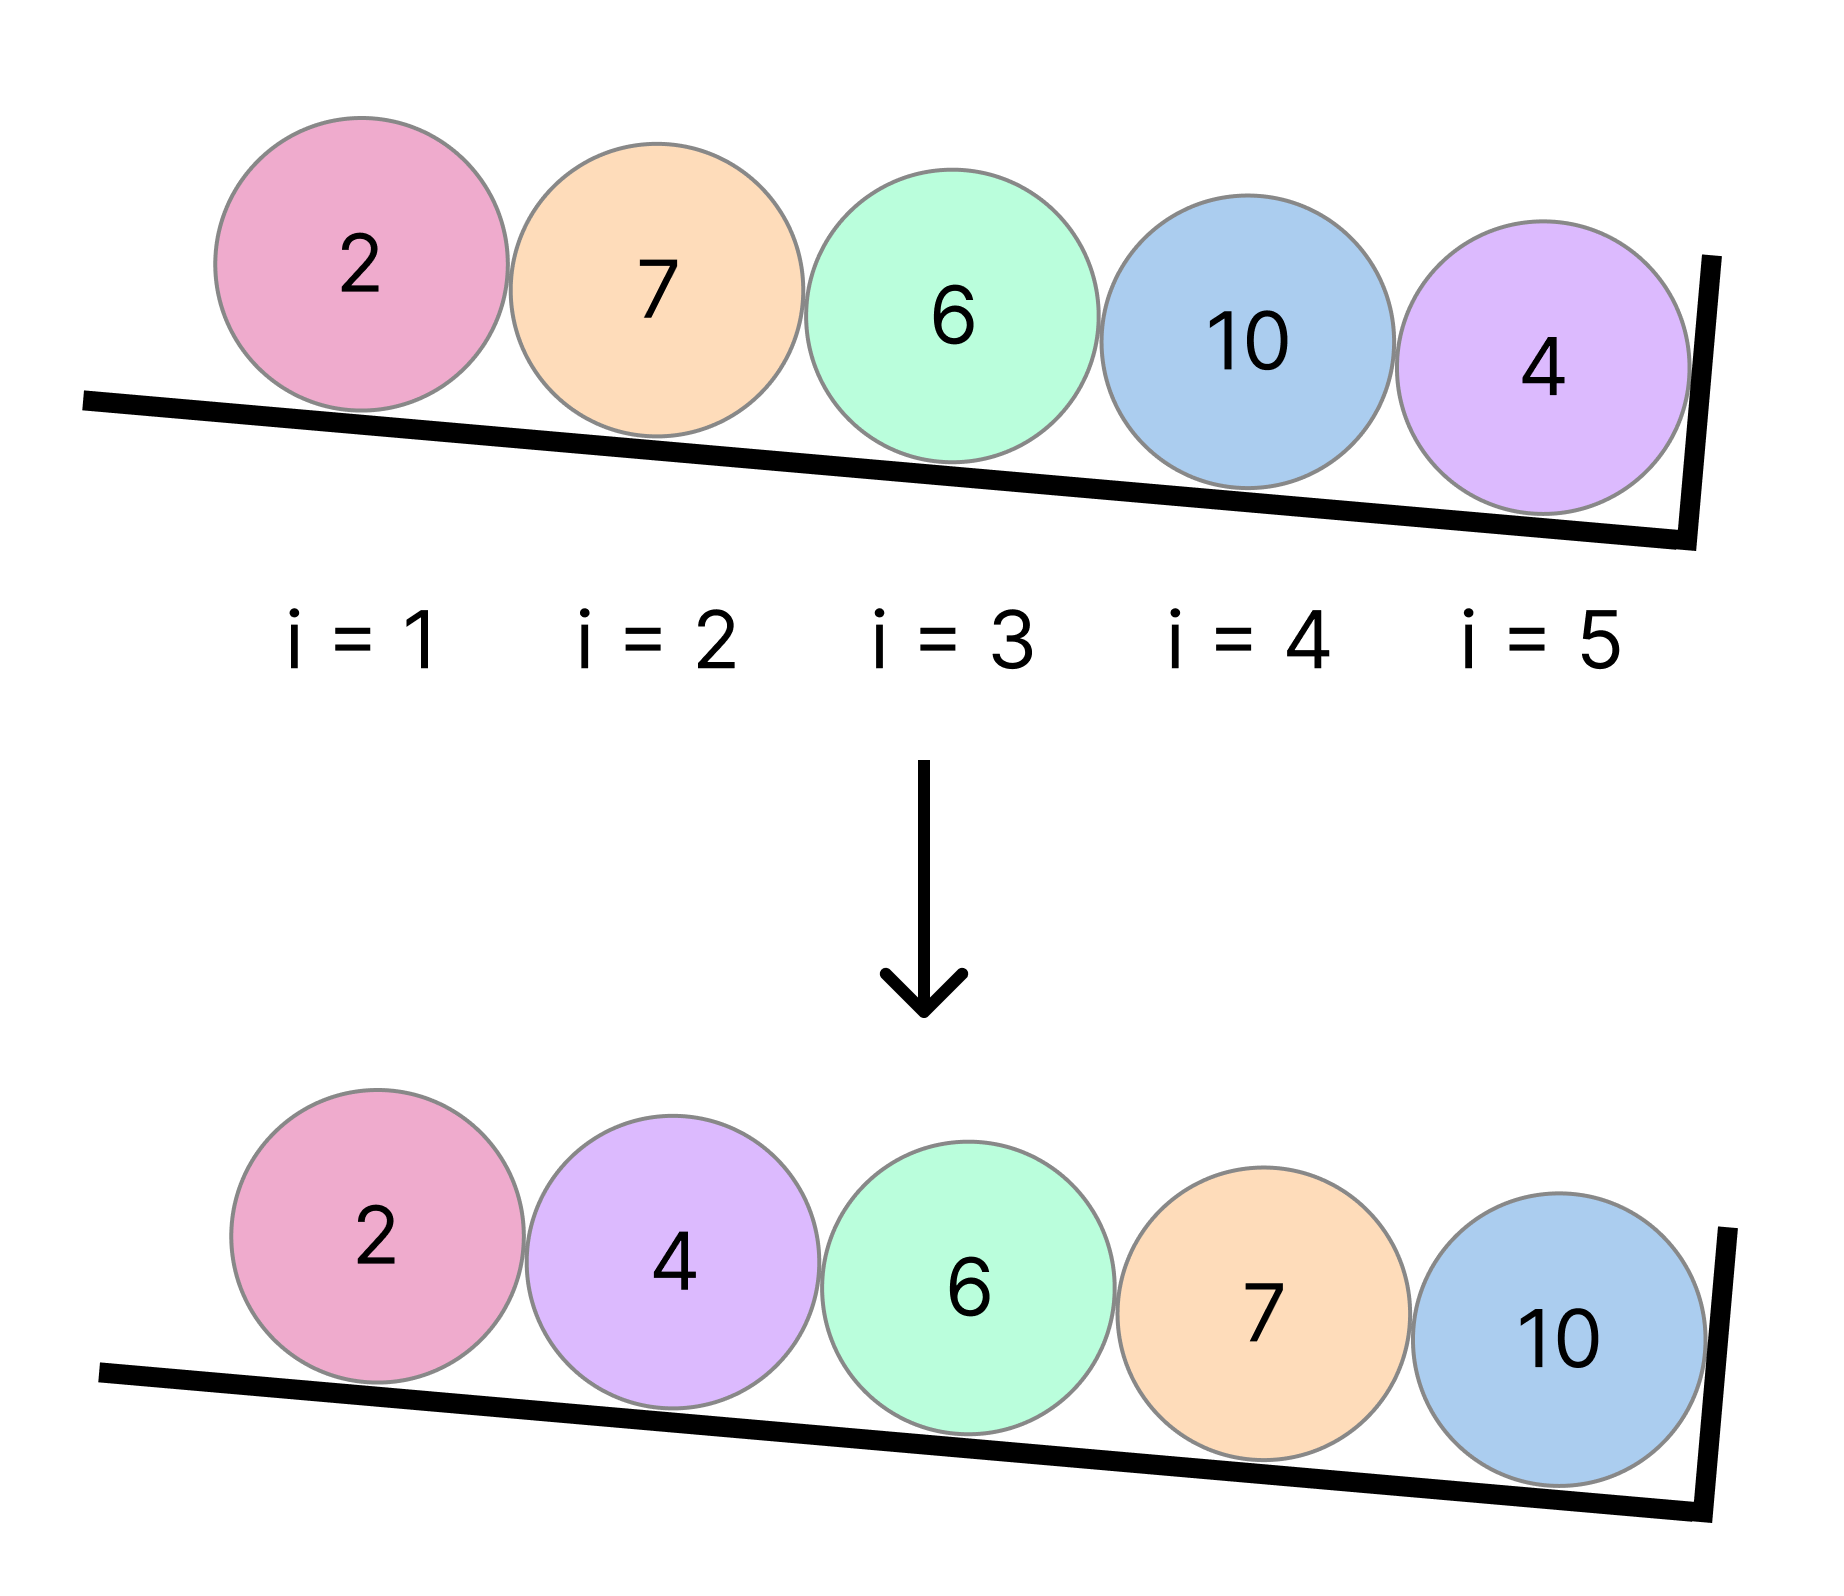
\includegraphics[width=0.5\textwidth]{../pictures/image.png} \\
\end{center}

건구스는 최대한 일찍 퇴근하기 위해 가장 적은 이동 횟수로 볼링공을 정리하고 싶다. 높은 위치부터 낮은 위치까지 레일에 놓여진 순서대로 $i$번째 볼링공 무게 $w_i\ ( 1 \le i \le N )$가 주어졌을 때, 건구스를 도와 최소 이동 횟수를 구하는 프로그램을 작성하자.


\InputFile
첫째 줄에 볼링공의 개수 $N\ ( 1 \le N \le 200\,000 )$이 주어진다.

둘째 줄에는 볼링공의 무게를 나타내는 정수 $w_i\ ( 1 \le i \le N,$ $1 \le w_i \le 1\,000\,000 )$가 공백으로 구분되어 주어진다.

\OutputFile
모든 볼링공을 정리한 후, 즉 모든 $i,\ j\ ( 1 \le i < j \le N )$에 대해 $w_i \le w_j$가 되도록 하는 최소 이동 횟수를 출력한다.

\Examples

\begin{example}
\exmp{
5
2 7 6 10 4
}{%
3
}%
\exmp{
7
2 3 2 3 1 2 4
}{%
3
}%
\exmp{
3
1 2 3
}{%
0
}%
\end{example}

\end{problem}
